\section{Einleitung}\label{sec:introduction}
\IEEEPARstart{S}{ysteme} zur Spracherkennung finden eine zunehmende Verbreitung und Beliebtheit im alltäglichen Leben. Das Spektrum dieser Anwendungen ist dabei Vielfältig und reicht vom Diktieren von Nachrichten über das Steuern von Geräten bis hin zum Einsatz in Autos. Dabei ist die Qualität der Spracherkennung und die Reaktion des Systems ein entscheidender Faktor, um die Interaktion so natürlich wie möglich zu gestalten \cite{Yu.2014}. Allerdings ergibt sich hier ein Hindernis für mehrsprachige Nutzer. Die natürliche Interaktion wird limitiert, da automatische Spracherkennungssysteme den Anwender auf eine voreingestellte Sprache beschränken. In den meisten herkömmlichen Systemen werden Sprachen sowie Dialekte unabhängig voneinander betrachtet. Es wird für jede Sprache ein separates akustisches Modell trainiert \cite{Gonzalez.2015}. Bei weltweit etwa 7000 gesprochenen Sprachen ist es daher nur konsequent, multilinguale Spracherkennungssysteme zu entwickeln \cite{Gary.2018}. Allerdings erfordert ein solches System einen entsprechenden Satz an markierten Trainingsdaten, um wiederkehrende Muster der Sprache zu erkennen. 
Dieser Umstand sorgt für erhebliche Qualitätsunterschiede zwischen den Sprachen, da nicht alle Sprachen über solche Datensätze verfügen. Um die Knappheit der beschrifteten Trainingsdaten zu kompensieren, wird der Ansatz der geteilten Hidden Layer genutzt \cite{Schultz.1998}. Dieser Ansatz stützt sich auf das Zusammenführen aller Daten, um so eine gemeinsame Nutzung der Phoneme zu gewährleisten. Phoneme stellen dabei eine abstrakte Repräsentation aller Laute einer Sprache dar \cite{Zissman.2001}. Um akustische Modelle für eine Vielzahl von Sprachen zu trainieren, um die Kosten, die beim Training dieser Modelle entstehen zu reduzieren und um neue Anwendungsszenarien zu unterstützen, besteht ein wachsendes Interesse an der Entwicklung mehrsprachiger Spracherkennungssysteme \cite{Yu.2014}.
\\\\
Zu Beginn erfolgt die Erläuterung des grundlegenden Aufbaus eines solchen Systems. Dabei werden die Unterschiede zu einem monolingualen System hervorgehoben. Darauf aufbauend wird erläutert, wie die Identifikation sowie die Erkennung von Sprachen funktioniert. Anschließend werden die Recurrent Neural Networks sowie deren Erweiterung, die Long Short Term Memory-Netzwerke (LSTM) beschrieben, welche heute im Bereich der multilingalen Spracherkennung verwendet werden. Dabei wird beleuchtet, wie dieses funktioniert und welche Vorteile gegenüber anderen tiefen neuronalen Netzen bestehen. Das Training eines solchen Modells folgt im Anschluss mit einer abschließenden Diskussion bezüglich weiterhin bestehender Probleme und zukünftiger Ansätze.

\section{Verwandte Arbeiten}
Dieses Kapitel stellt exemplarisch wichtige Arbeiten vor, welche mit dem Thema des Artikels in Beziehung stehen. Es gibt viele Forschungsarbeiten auf dem Gebiet der mehrsprachigen und sprachübergreifenden Spracherkennung. Der Artikel konzentriert sich allerdings nur auf diejenigen, die Recurrent Neural Networks bzw. LSTM-Netzwerke verwenden. Der Schwerpunkt dieser Arbeit liegt bei dem Untersuchen dieser Verfahren zur Realisierung entsprechender Systeme sowie die sich hier ergebenden Vorteile gegenüber bisheriger Verfahren. Dabei wird kein detaillierter Vergleich verschiedener Modelle aufgeführt. \\ 
Die Abhandlung lehnt an das Werk Automatic Speech Recognition - A Deep Learning Approach von Dong Yu und Li Deng \cite{Yu.2014} an. Die Grundlagen bezüglich automatischer Spracherkennungssysteme, konventioneller Ansätze und Trainingsverfahren sowie die Architektur mehrsprachiger Systeme werden hier beschrieben.
Ein weiteres für diesen Artikel interessantes Werk ist das Buch Sprachverarbeitung von Beat Pfister und Tobias Kaufmann, in welchem Grundlagen und Methoden der Sprachsynthese und Spracherkennung genau beschrieben werden.  
Des Weiteren wird in \cite{2017arXiv170307090T} von Tian et al. ein alternatives LSTM-Netzwerk vorgeschlagen, welches den konventionellen Ansatz übertrifft. Auch in den Arbeiten von Graves et al. {\cite{6638947}} und Sak et al. \cite{2014arXiv1402} werden Recurrent Neural Networks im Bezug auf Spracherkennung untersucht. Dabei wird ebenfalls die Effizienz von LSTM-Netzwerken unter anderem durch Experimente bestätigt. \\Da vor allem Sprachen mit einem geringen Satz an Trainingsdaten zu Problemen bei Spracherkennungssystemen führen, ist das Multitask Learning (MTL) ein wichtiger Ansatz multilingualer Sprachsysteme. In der Arbeit von Lu et al. \cite{multitask} werden daher verschiedene Methoden des MTL vorgeschlagen. In dem Artikel wird belegt, dass das Verfahren den Mangel an Ressourcen kompensieren kann, indem auf gemeinsam erlernte Inhalte zurückgegriffen wird.


\section{Hintergrund}
Ein multilinguales Spracherkennungssystem besteht aus mehreren Komponenten. Abbildung \ref{fig:pipeline} illustriert dabei die Pipeline dieser Module. Die Erkennung der Sprache funktioniert über das Aufnehmen von Schallwellen, die beim Sprechen produziert werden. Diese lassen sich über einen elektroakustischen Wandler (Mikrophon) in ein elektrisches Signal umwandeln. Das elektrische Tonsignal wird daraufhin digitalisiert bzw. in Bits konvertiert (Sampling) und über Vorverarbeitung entsprechend aufbereitet, um es in ein neuronales Netz zu speisen {\cite{beat_tobias}}. Diese Daten lassen sich anschließend in Sequenzen aufteilen, aus denen die benötigten Features extrahiert werden. Abbildung \ref{fig:pipeline} stellt diesen Teilschritt als Spektrogramm dar, welches das gesamte Frequenzspektrum visualisiert. Die Feature-Vektoren müssen hier so gewählt werden, dass die kleinste, effizienteste Menge für die Sprachverarbeitung herausgefiltert wird. Die gewonnenen Features dienen schließlich als Eingabe für die Sprachidentifikation. Die gewonnene Information bezüglich der gesprochenen Sprache kombiniert mit den Features werden als Eingabe für den Decoder genutzt. Unter Zuhilfenahme des akustischen Modells sowie des Sprach- und Lexikalmodells, wird der gesprochene Text analysiert und klassifiziert. Die drei Modelle werden von Bäckström \cite{Tom.2016} wie folgt beschrieben:

\begin{itemize}
    \item \textit{Akustikmodell.} Die Menge an Daten, die das neuronale Netz darüber informiert wie die Zusammenhänge zwischen Phonemen und einem konkreten Audiosignal sind. Die Phoneme können
    sowohl kontextabhängig als auch kontextfrei sein.
    Erlernt wird das Modell durch Audioaufnahmen und den zugehörigen Abschriften – die akustischen Trainingsdaten.
    \item \textit{Lexikalmodell.} Dieses Modell bildet eine Sequenz von Phonemen, die durch das Akustikmodell gewonnenen werden, auf gültige Wörter einer Sprache ab. Hierfür werden textuelle Trainingsdaten eingesetzt.
    \item \textit{Sprachmodell.} Die Wahrscheinlichkeit für einen syntaktisch und semantisch korrekten Satz wird genutzt, um aus einer Reihe von Wörtern, die durch das Lexikalmodell gewonnen werden, gültige Wortsequenzen bzw. Sätze zu bilden.
    Beispielsweise folgt auf das englische Wort 'thank' mit einer hohen Wahrscheinlichkeit das Wort 'you' oder
    'god'. Für das Training dieses Modells werden textuelle Trainingsdaten eingesetzt.
\end{itemize}

Jedes dieser drei Modelle muss separat trainiert werden. Das führt zu einer erhöhten Komplexität, verglichen mit dem Trainieren eines einzelnen, gemeinsamen Modells.
Darum wird in den letzten Jahren vermehrt der Ansatz verfolgt, Ende-zu-Ende-Systeme zu entwickeln. Dabei werden die drei Modelle als ein System trainiert und eingesetzt.
Chan et al. \cite{Chan.2015} und Prabhavalkar et al. \cite{Prabhavalkar.2017} zeigen hierzu verbesserte Ergebnisse, verglichen mit mehreren Systemen welche auf einzelne Modelle bauen.

\begin{figure}[h!]
    \centering
    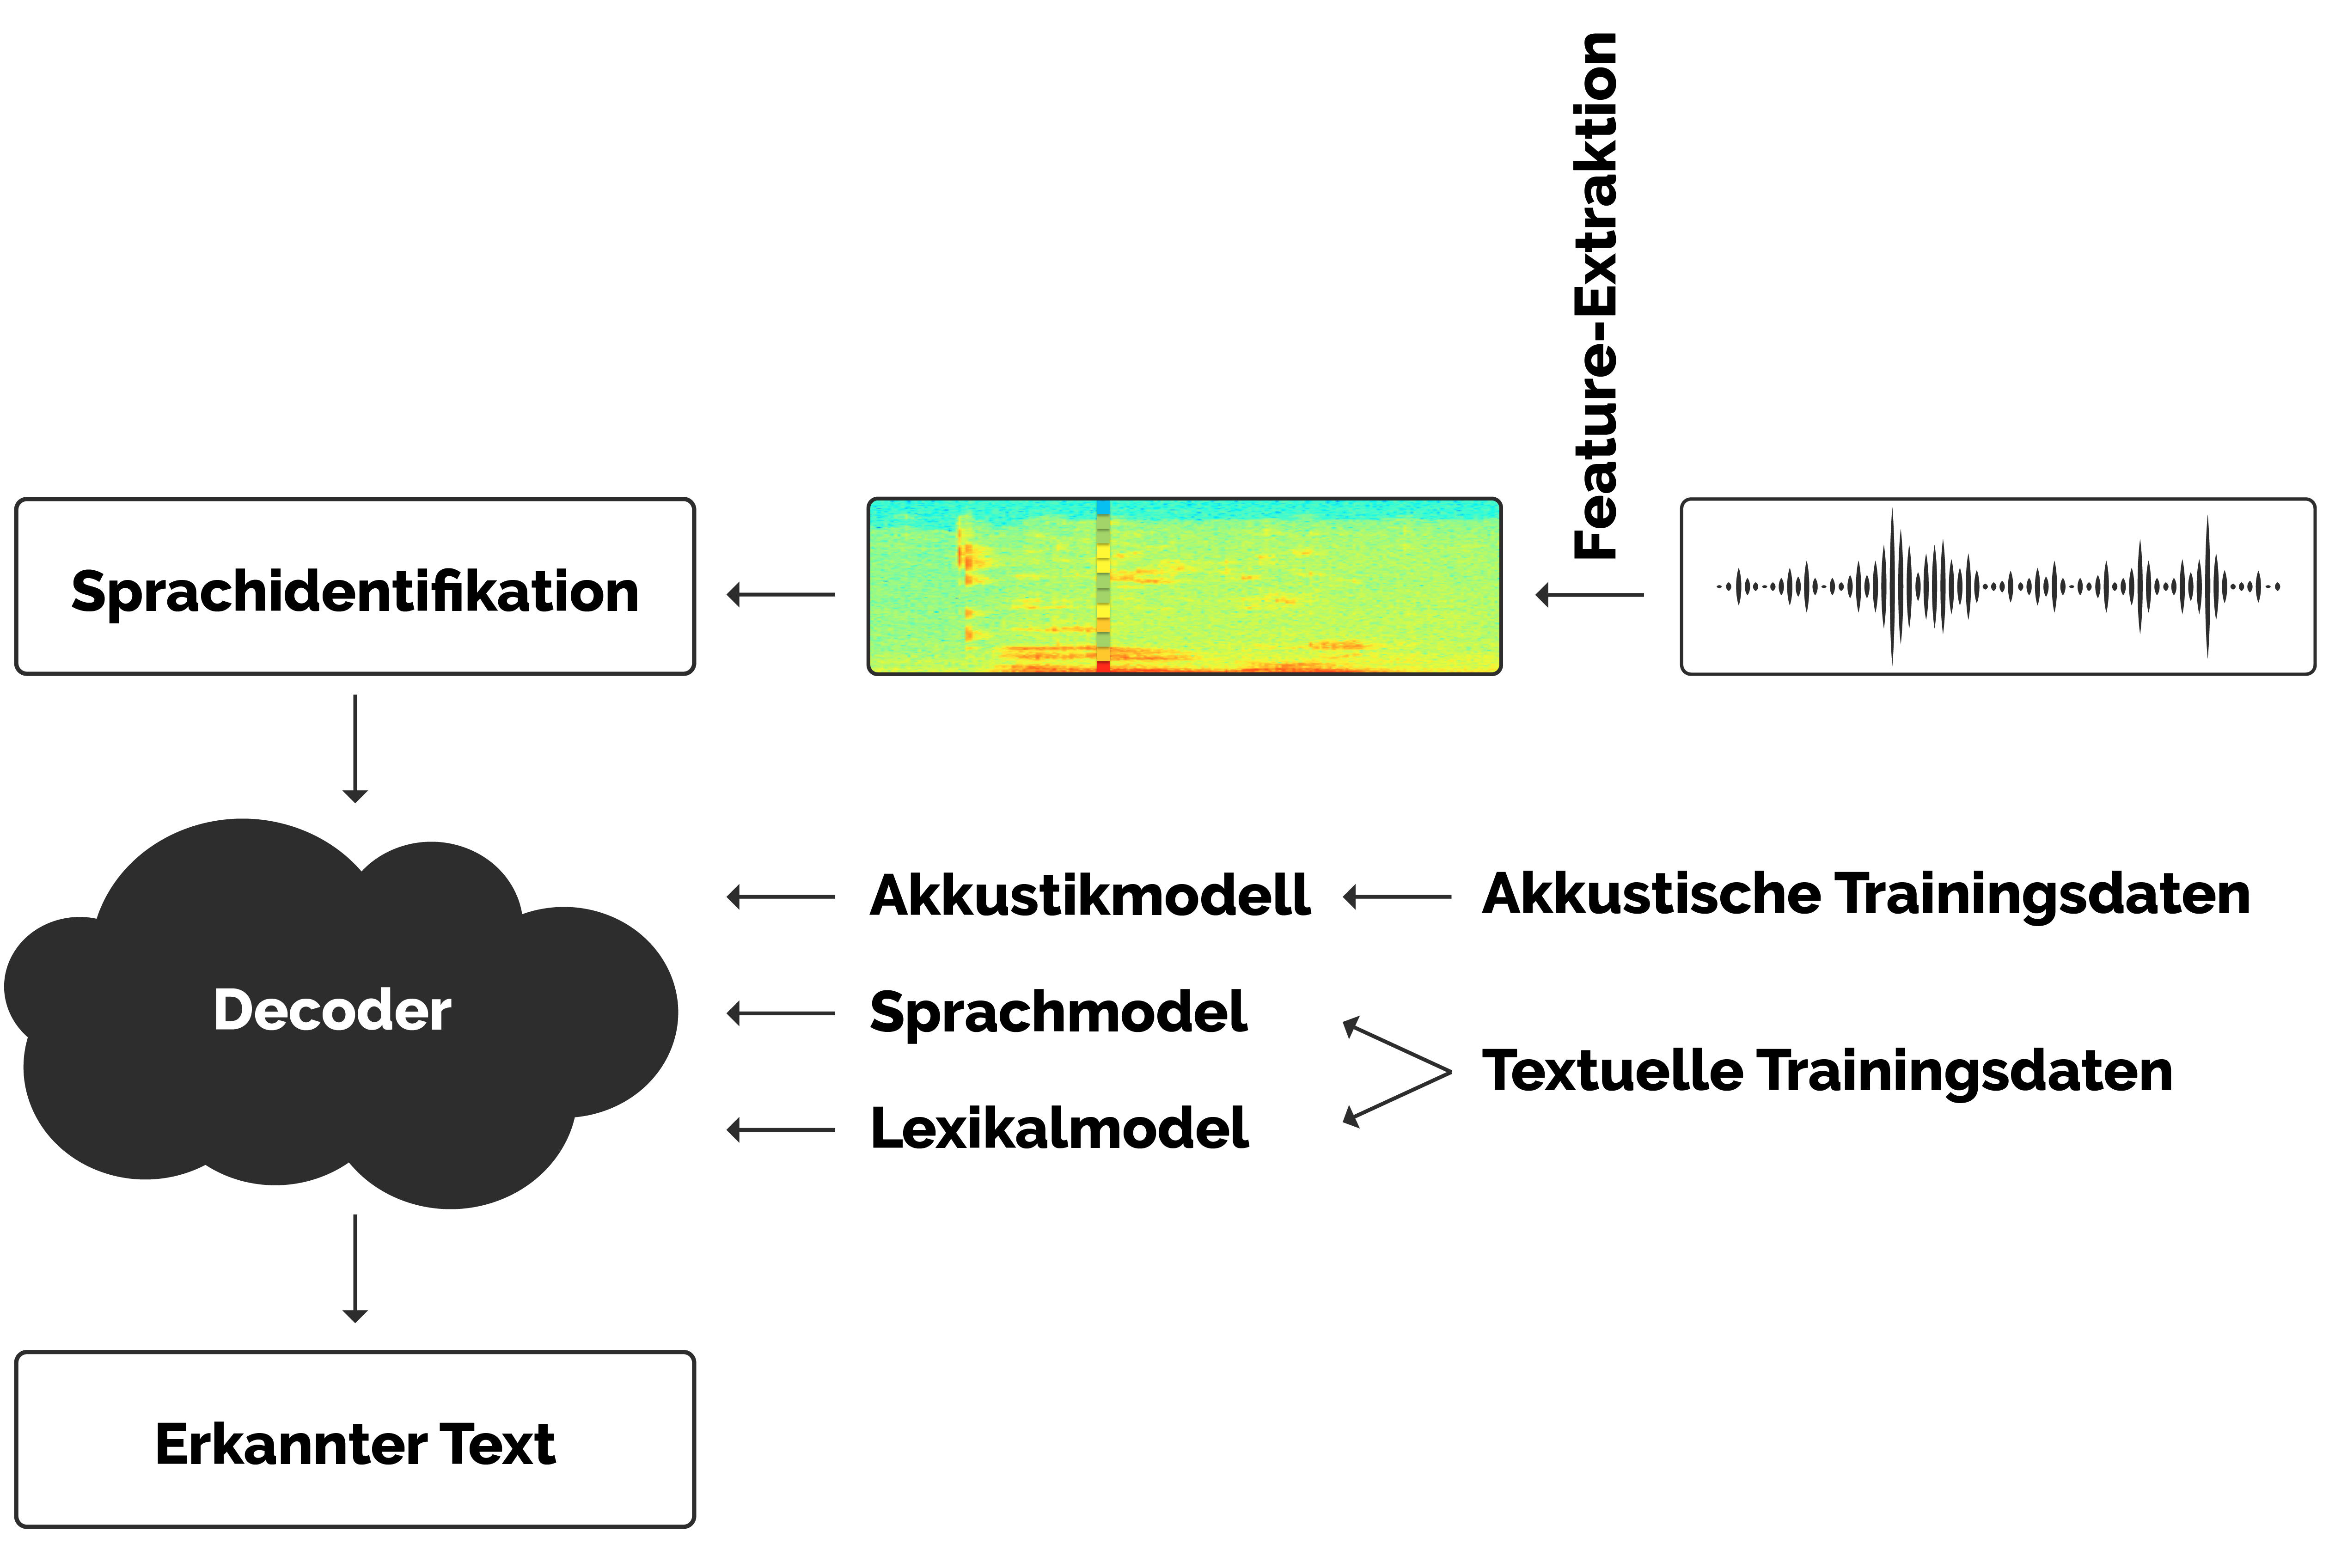
\includegraphics[width=1\linewidth]{images/pipeline}
    \caption{Pipeline eines Spracherkennungssystems (Eigene Darstellung, in Anlehnung an: \cite{Tom.2016}) }%\cite{??}}
    \label{fig:pipeline}
\end{figure}